\documentclass[fleqn, letterpaper]{amsart}
%\documentclass[letterpaper]{tufte-handout}
%\usepackage{times}
\usepackage{amsmath}
\usepackage{amssymb}
\usepackage{graphicx}
\usepackage{booktabs}
\usepackage{multirow}
\usepackage{listings}
\usepackage{epstopdf}
\usepackage{bm}
%\usepackage[left=1in]{geometry}

\newcommand{\R}{\mathcal{R}}
\newcommand{\E}{\text{E}}
\newcommand{\p}{p_{XY}}
\newcommand{\T}{^\text{T}}
\newcommand{\y}{\mathbf{y}}
\newcommand{\z}{\mathbf{z}}
\newcommand{\I}{\mathbf{I}}
\newcommand{\HH}{\mathbf{H}}
\newcommand{\A}{\mathbf{A}}
\newcommand{\GG}{\mathbf{G}}
\newcommand{\vecy}{\mathbf{y}}
\newcommand{\uu}{\mathbf{u}}
\newcommand{\cyy}{\mathbf{C}_{yy}}
\newcommand{\cyz}{\mathbf{C}_{yz}}
\newcommand{\czz}{\mathbf{C}_{zz}}
\newcommand{\cuu}{\mathbf{C}_{uu}}
\newcommand{\cvv}{\mathbf{C}_{vv}}
\newcommand{\cpp}{\mathbf{C}_{\psi\psi}}
\renewcommand{\arraystretch}{1.5}
\renewcommand{\vec}[1]{\mathrm{#1}}

\title{Course Project --- ENCE689E Spring 2014}
\author{David Prentiss}

\begin{document}
\maketitle

\section{Project Summary}

The Famine Early Warning System Network (FEWSNET) project is a federally funded effort to monitor regional and global economies, food, and climate in order to provide advanced warning of humanitarian, food related disasters.
Among the many FEWSNET tools is a model of pastoral herds. This model is an aid to the analysis of food security in regions where pastoral livelihoods are prevalent. While it sees wide adoption among food security analysts, its statistical properties are not well investigated. Furthermore it may be possible to enhance this model with adaptive filtering techniques. This work investigates the model's general charachteristics and assess the skill of the Ensemble Kalman Filter for data assimilation in a synthetic twin experiment.

\section{Herd Dynamics Model}

The herd dynamics model predicts the size and demographic features of a hypothetical herd from season to season based on the previous season's rainfall amount and quality.
These demographic features are sub--groups related to sex and reproductive capacity where individuals are categorized as either adult female, newborn, young female, or young male.
As such, the state of the herd at each season $t$, where $t$ is an index of sequential seasons is captured by the state vector $\vecy_t$.
The elements of $\vecy_t$ are the head--counts of individuals in each sub--group at the beginning of season $t$.
\begin{align}
y_{\text{AF}}^{t+1} &= [y_{\text{AF}}^t + y_{\text{YF}}^t - f_{\text{SF}}^ty_{\text{AF}}^t - f_{\text{MM}}^ty_{\text{AF}}^t]w_{\text{AF}}\\
y_{\text{NB}}^{t+1} &= [f_{\text{C}}^ty_{\text{AF}}^t]w_{\text{NB}}\\
y_{\text{YF}}^{t+1} &= [0.5(y_{\text{NB}}^t - f_{\text{MI}}^ty_{\text{NB}}^t) - f_{\text{MM}}^ty_{\text{YF}}^t]w_{\text{YF}}\\
y_{\text{YM}}^{t+1} &= [y_{\text{YM}}^t + y_{\text{NB}}^t - y_{\text{YF}}^{t+1} - f_{\text{SM}}^ty_{\text{YM}}^t - f_{\text{MM}}^ty_{\text{YM}}^t]w_{\text{YM}}
\end{align}
where $f_{\text{C}}^tf$, $f_{\text{SM}}^t$, $f_{\text{SF}}$, $f_{\text{MM}}$, and $f_{\text{MI}}$ are the rates of conception, male sales, female sales, mature mortality, and immature mortality respectively and
$w_{\text{C}}^tf$, $w_{\text{SM}}^t$, $w_{\text{SF}}$, $w_{\text{MM}}$, and $w_{\text{MI}}$
Step super--scipts and arguments have been omitted for clarity.
\begin{itemize}
\item $w$ are multiplicative model error.
\item $w\sim\ln\mathcal{N}(\mu,\sigma)$, $\bar{w}=1$, $\sigma_w^2 = 0.001$.
\item Multiplicative, lognormal error avoids negative values.
\item It also means we cannot use the KF.
\end{itemize}
See figure \ref{rferels}.
\begin{figure}
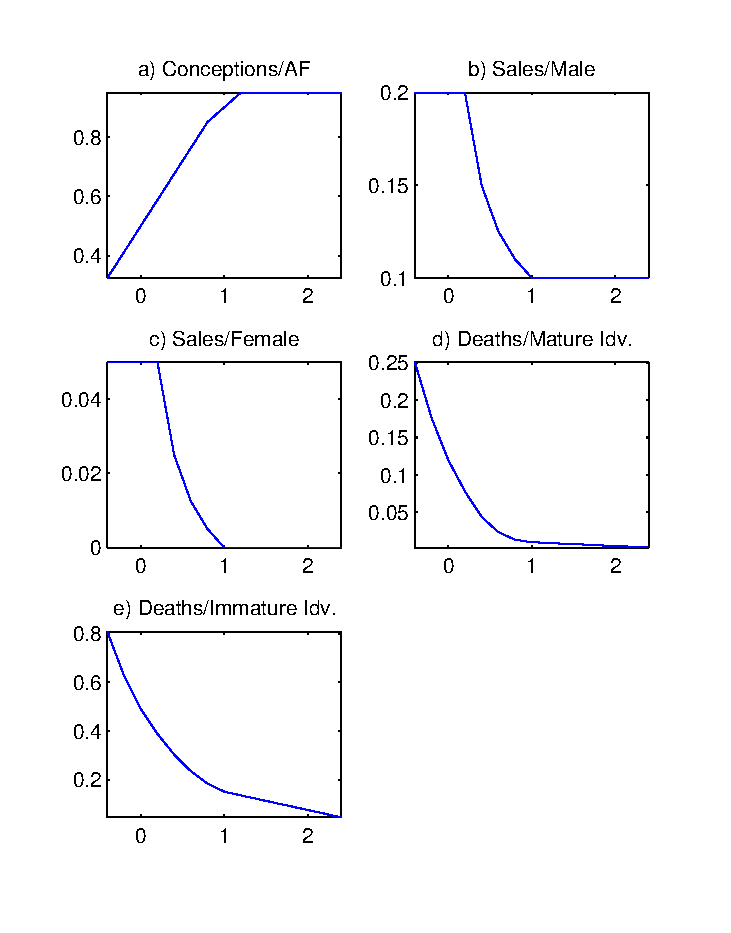
\includegraphics[width=1.0\textwidth]{refrel}
\label{rferels}
\end{figure}
\section{Model Dynamics}
The herd dynamics model is unproven and under--analyzed. In order to asses the efficacy of data assimilation techniques, it will first be useful to account for model behavior in general. To that end, the following items will be considered to judge the model's general dynamic characteristics and sensitivities. 
\begin{itemize}
  \item General tendencies vis--a--vis damped and un--damped dynamics. A variety of true forcings and initial conditions will be modeled to determine any thresholds between stable and unstable behavior.
  \item Sensitivity to initial herd size. Initial results suggest herd size has little effect on overall herd dynamics. Randomly chosen herd sizes will be compared to confirm this.
  \item Sensitivity to initial herd demographics. Randomly chosen proportions of demographic sub--groups of herds with a fixed size will be compared.
  \end{itemize}
\section{Data Assimilation}
The model, in its current form, is linear and little is know about its error characteristics. As it stands, a standard Kalman Filter might be used for data assimilation under a Gaussian error assumption. However, given that biological systems are often nonlinear and that the forcings are base on precipitation amounts and timings, both the linear dynamic and Gaussian assumptions may, after future updates to the model, be inappropriate. Thus the skill of the Ensemble Kalman Filter in this context will be assessed against the following objectives:
\begin{itemize}
  \item Recovery of initial conditions (size and proportion). A synthetic twin experiment with a wide range of initial condition error will be conducted.
  \item Sensitivity of skill to ensemble size. The synthetic experiment will be repeated for various ensemble sizes.
  \item Sensitivity of skill to model error variance. The synthetic experiment will be repeated for multiple values of the model error variance.
  \end{itemize}

\section{General Characteristics}

\begin{figure}
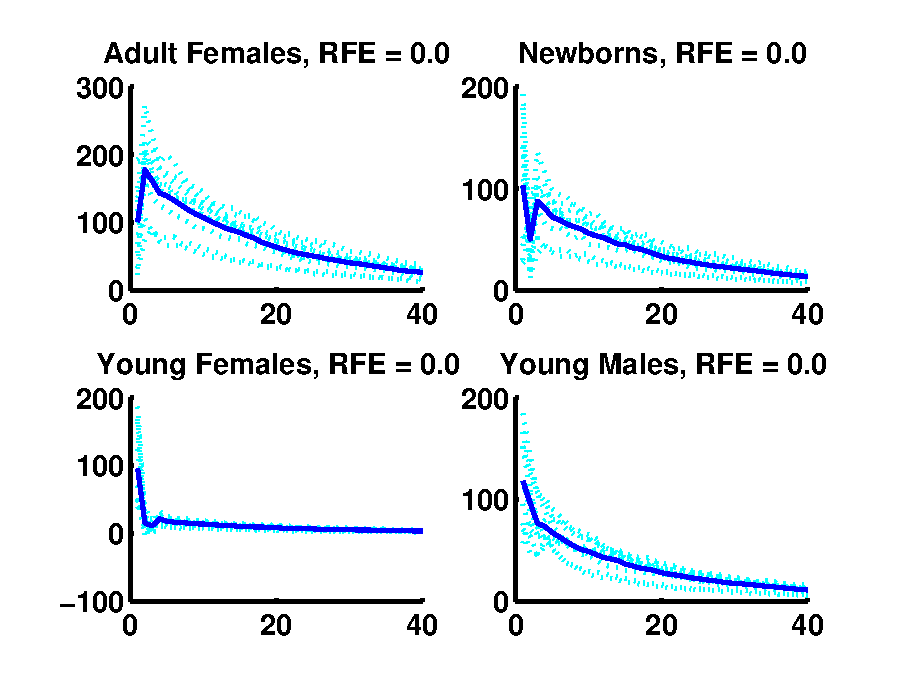
\includegraphics[width=\textwidth]{general0}
\end{figure}
\begin{figure}
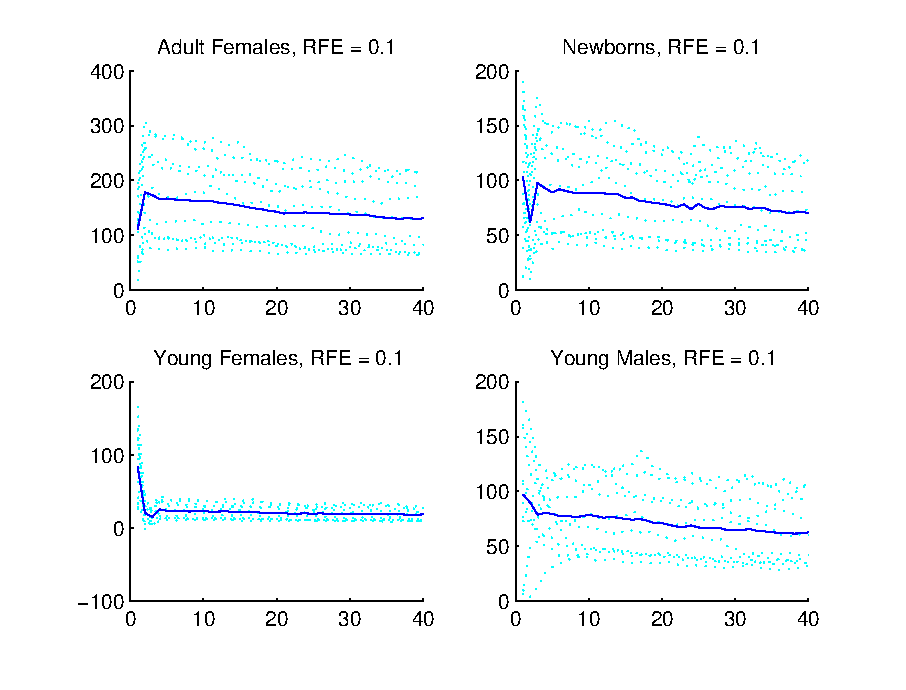
\includegraphics[width=0.9\textwidth]{rgeneral1}
\end{figure}
\begin{figure}
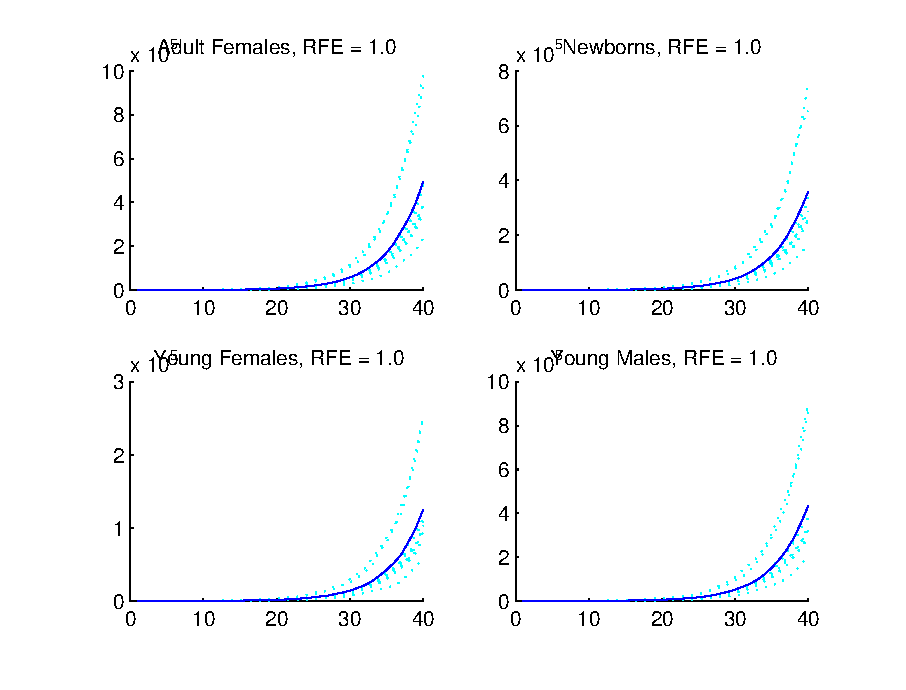
\includegraphics[width=0.9\textwidth]{rgeneral10}
\end{figure}
\begin{figure}
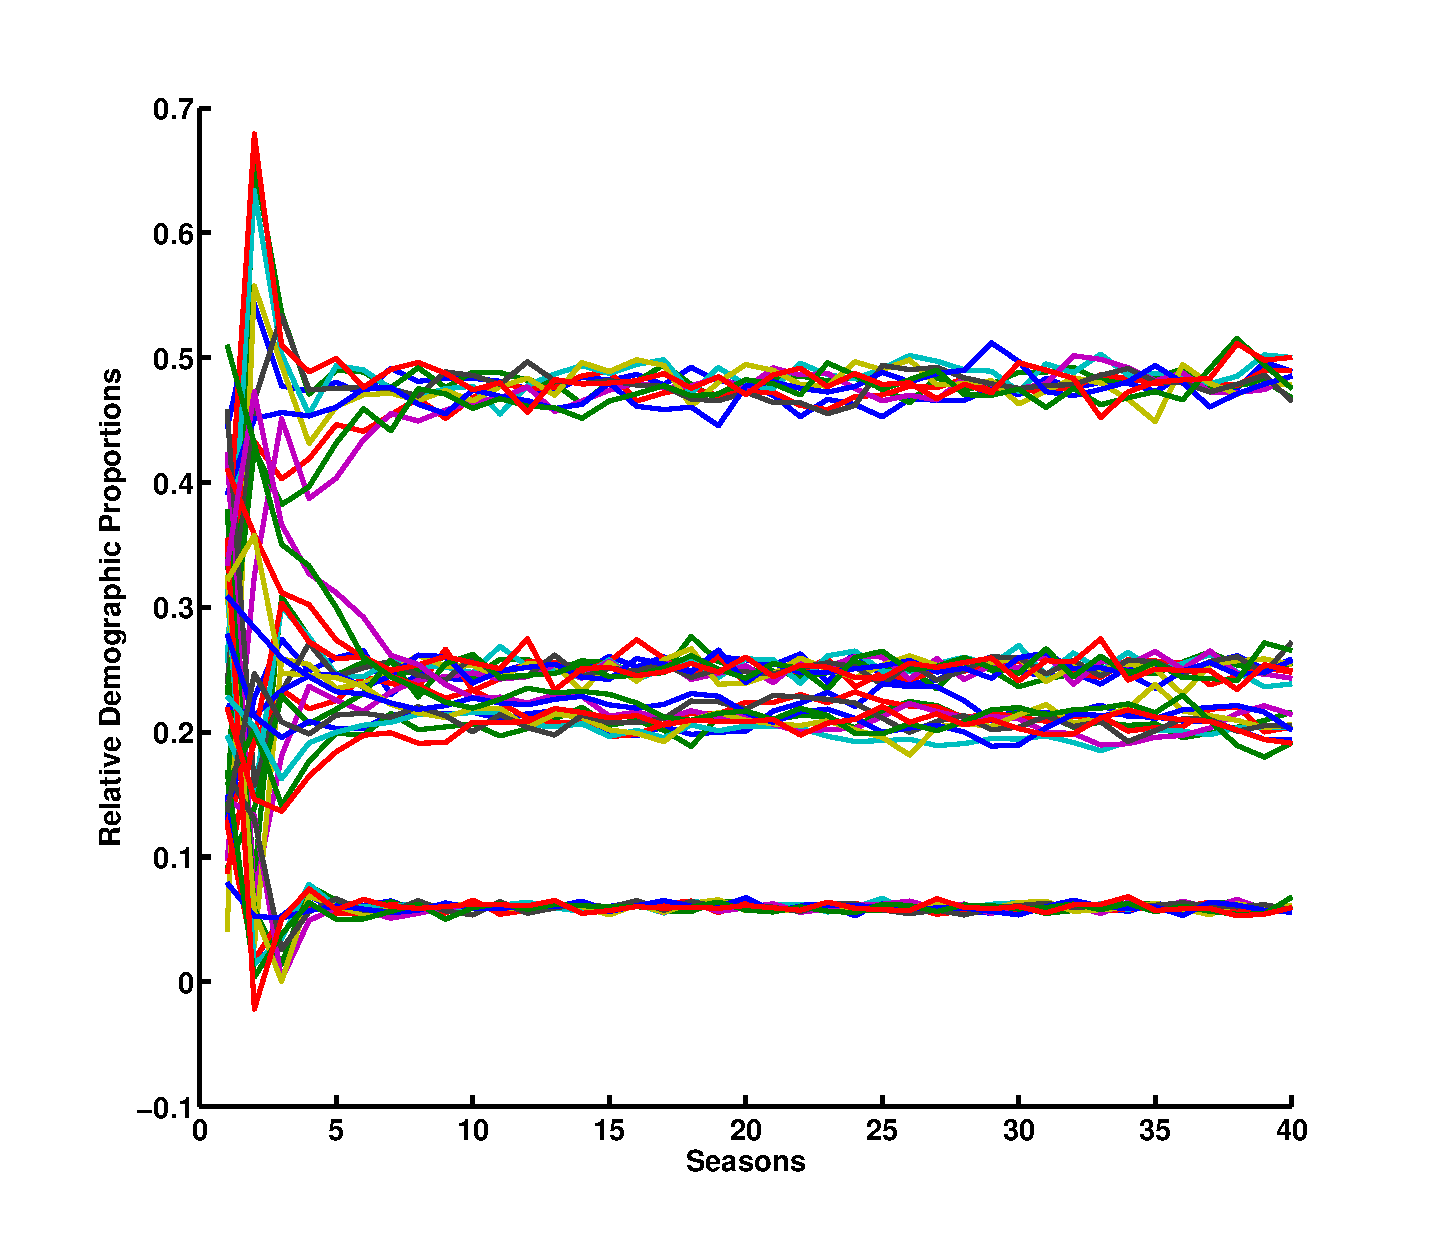
\includegraphics[width=0.9\textwidth]{relprop}
\end{figure}
\section{Data Assimilation}
\subsection{Synthetic Truth}
\begin{figure}
\begin{center}
\includegraphics[width=0.9\textwidth]{rforcing}
\end{center}
\end{figure}
\subsection{Initial Conditions}

\begin{itemize}
\item True initial conditions: $(50\ 10\ 10\ 5)^T$
\item Ensemble initial conditions: $y_0\sim\mathcal{U}(0,200)$, uncorrelated
\item 100--member ensemble initial mean: $(95\ 94\ 101\ 98)^T$
\item 100--member ensemble initial covariance:

$\left(\begin{array}{cccc} 3345.0 & -515.0 & 220.6 & -144.6\\ -515.0 & 2995.0 & -665.7 & -53.02\\ 220.6 & -665.7 & 3431.0 & 72.85\\ -144.6 & -53.02 & 72.85 & 3061.0 \end{array}\right)$
\end{itemize}

\begin{figure}
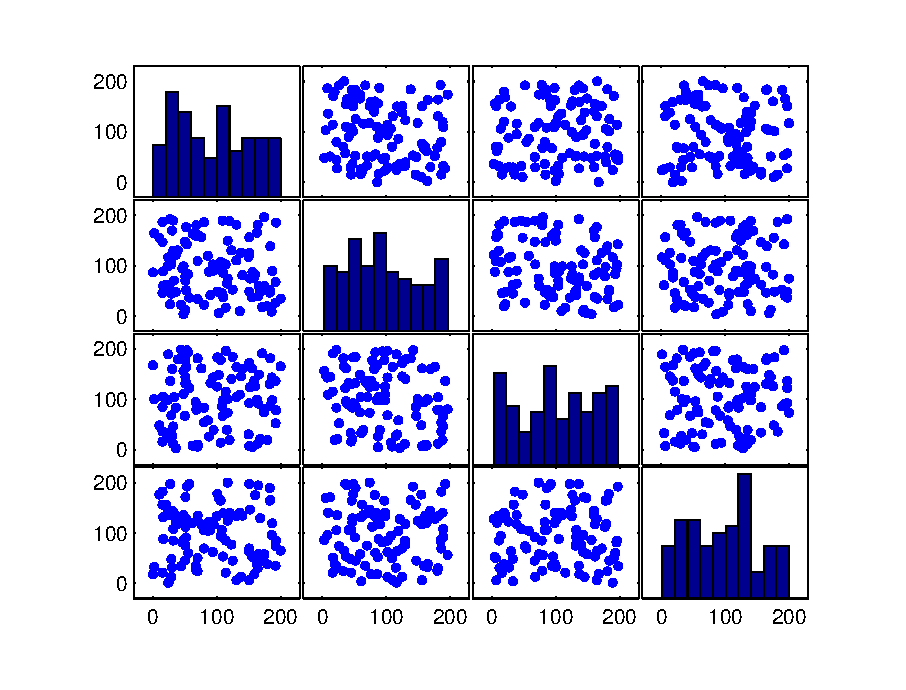
\includegraphics[width=1\textwidth]{rinitcov}
\end{figure}
\begin{figure}
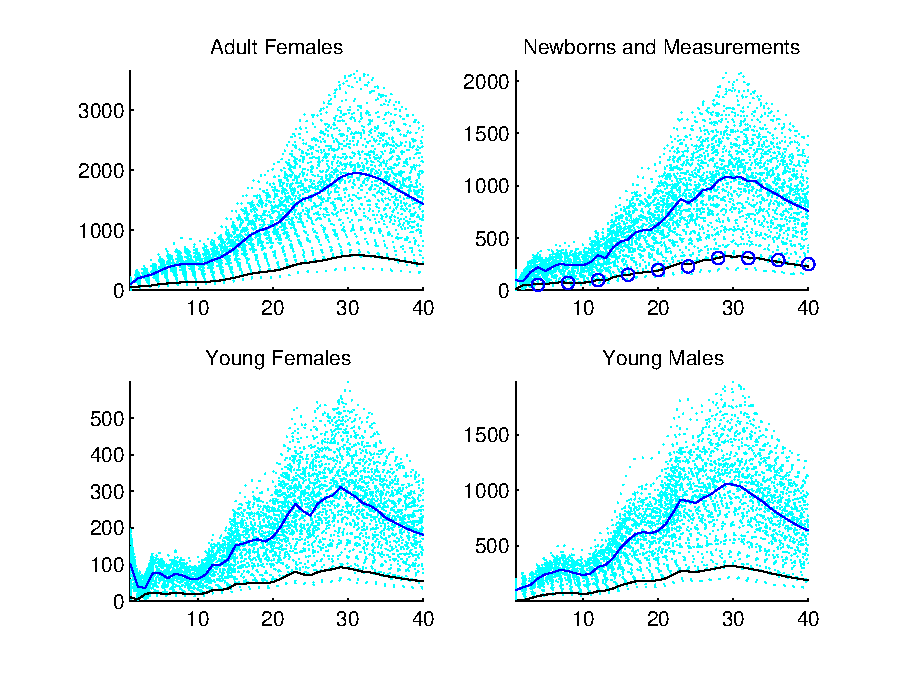
\includegraphics[width=1\textwidth]{ropenloop}
\end{figure}
\begin{figure}
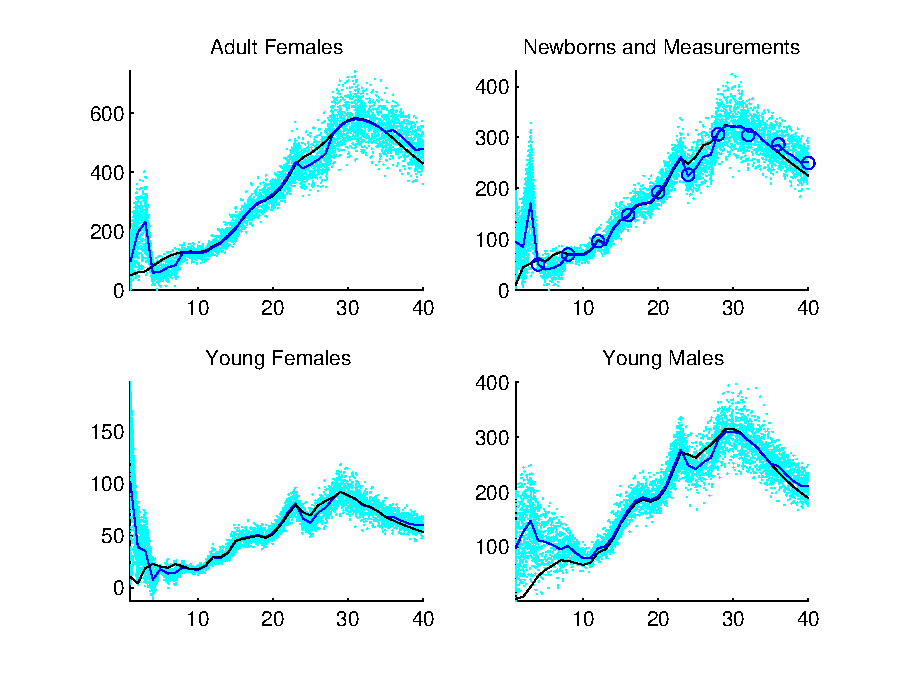
\includegraphics[width=1\textwidth]{kf}
\end{figure}
\begin{figure}
\includegraphics[width=1\textwidth]{rol30cov}
\end{figure}
\begin{figure}
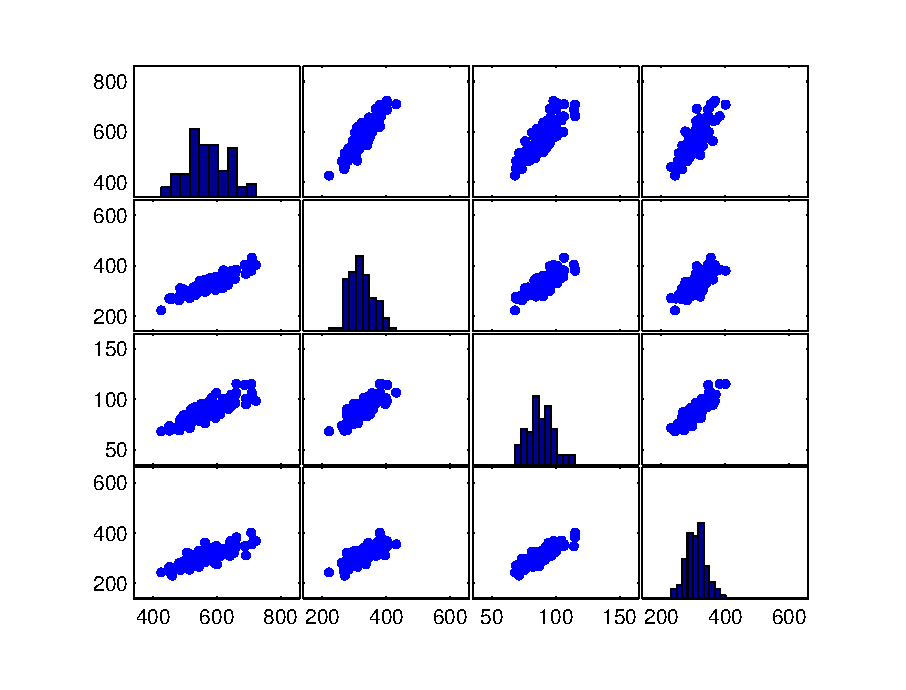
\includegraphics[width=1\textwidth]{rkf30cov}
\end{figure}
\begin{table}
\begin{tabular}{rrr}
& Bias & RMSE \\
\hline
Open loop & 441.2 & 565.2 \\
EnKF & 6.5 & 31.1
\end{tabular}
\caption{Skill of open loop vs. EnKF}
\end{table}

\subsection{Ensemble Size}

\begin{table}
\begin{tabular}{rrrr}
Ensemble members & 10 & 100 & 1000 \\
\hline
Bias & 10.5 & 6.5 & 6.5 \\
RMSE & 36.3 & 31.1 & 31.7
\end{tabular}
\caption{Skill for various ensemble sizes}
\end{table}

\subsection{Model Error Variance}

\begin{table}
\begin{tabular}{rrrr}
Model Error Variance & 0.001 & 0.01 & 0.1 \\
\hline
Bias & 6.5 & 7.2 & 9.7\\
RMSE & 31.1 & 30.9 & 40.7
\end{tabular}
\caption{Skill for various model error variances}
\end{table}

%\bibliographystyle{plainnat}
%\bibliography{project}
\end{document}
